\documentclass[8pt,a4paper]{beamer}
\usepackage{graphicx} % Required for inserting images
\usepackage{color, colortbl}

\usepackage[english,serbian]{babel}
\usepackage{indentfirst}
\usepackage{verbatim}
\usepackage{fontspec}
\usepackage{polyglossia}
\usepackage{serbian}

\usepackage{booktabs}
\usepackage{tikz}
\usetikzlibrary{arrows.meta, positioning}




\usetheme{Szeged}
\usecolortheme{seahorse}

\title{Klasifikacija slika pasa i mačaka primenom dubokog učenja}
\author{Alma Hodžić, Mina Ristić}
\institute{Mašinsko učenje \\ Matematički fakultet \\ Univerzitet u Beogradu}
\date{\today}


\begin{document}

\begin{frame}
\titlepage

\begin{figure}[h!]
    \centering
    \begin{flushleft}
    \IfFileExists{slika1.jpg}{\includegraphics[width=15mm]{slika1.jpg}}{}
    \end{flushleft}
\end{figure}
\end{frame}

\begin{frame}{Sadržaj}
\tableofcontents
\end{frame}

\section{Uvod}

\begin{frame}{Uvod}
\begin{itemize}
    \item Cilj projekta je binarna klasifikacija slika pasa i mačaka primenom konvolutivnih neuronskih mreža. \pause
    \item Implementirana su i upoređena tri pristupa rastuće složenosti: \pause
    \begin{itemize}
        \item baseline CNN (VGG-6) treniran od nule \pause
        \item transfer learning sa VGG-16 mrežom treniranom na ImageNet skupu \pause
        \item fine-tuning poslednjeg konvolucionog bloka VGG-16 mreže \pause
    \end{itemize}
    \item Pored performansi, analizirana je i \textbf{interpretabilnost} modela --- vizualizacija međuslojnih aktivacija i Grad-CAM. \pause
    \item Projekat je inspirisan radom \textit{Lin, Household Animals Classification Using Deep Learning}, Stanford CS230, 2020.
\end{itemize}
\end{frame}

\section{Skup podataka}

\begin{frame}{Skup podataka --- Dogs vs. Cats}
\begin{columns}
\begin{column}{0.52\textwidth}
\begin{itemize}
    \item \textbf{25.000} označenih slika: 12.500 mačaka i 12.500 pasa --- savršeno balansiran skup. \pause
    \item Slike su prikupljene sa interneta, pa su vrlo raznolike:
    \begin{itemize}
        \item širina 42--1050 px (prosek 404)
        \item visina 32--768 px (prosek 360)
    \end{itemize} \pause
    \item Provereno: \textbf{0 oštećenih} fajlova, svih 25.000 u RGB formatu. \pause
    \item Sve slike se skaliraju na \textbf{224\,$\times$\,224\,$\times$\,3} --- ulaznu dimenziju VGG-16 mreže.
\end{itemize}
\end{column}
\begin{column}{0.46\textwidth}
    \begin{figure}[h!]
        \centering
        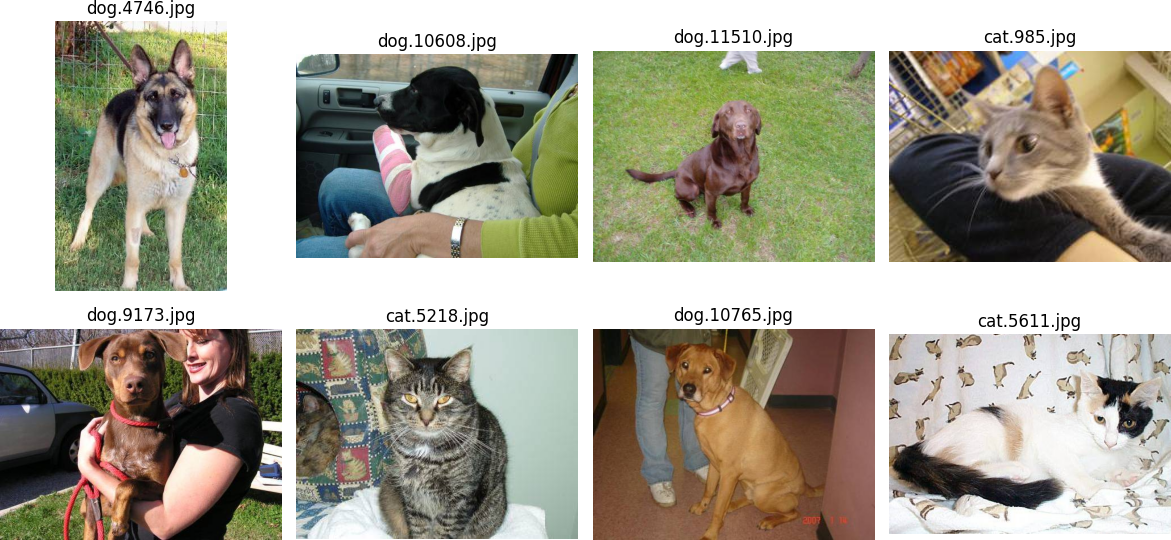
\includegraphics[width=\textwidth]{img/primeri.png}
    \end{figure}
\end{column}
\end{columns}
\end{frame}

\begin{frame}{Podela podataka}
\begin{columns}
\begin{column}{0.52\textwidth}
\begin{table}
\centering
\begin{tabular}{lrrr}
\toprule
\textbf{Skup} & \textbf{Slika} & \textbf{Mačke} & \textbf{Psi} \\
\midrule
Train      & 20.000 & 10.000 & 10.000 \\
Validation &  4.000 &  2.000 &  2.000 \\
Test       &  1.000 &    500 &    500 \\
\midrule
\textbf{Ukupno} & \textbf{25.000} & \textbf{12.500} & \textbf{12.500} \\
\bottomrule
\end{tabular}
\end{table}
\vspace{0.5\baselineskip}
\begin{itemize}
    \item Podela je \textbf{stratifikovana}, sa fiksiranim seed-om 42. \pause
    \item Napravljena je \textbf{jednom} i sačuvana u \texttt{split.csv} --- svi modeli koriste identične podatke, pa je poređenje pošteno. \pause
    \item Test skup se koristi \textbf{isključivo} za finalnu evaluaciju --- ne za trening ni za izbor hiperparametara.
\end{itemize}
\end{column}
\begin{column}{0.46\textwidth}
    \begin{figure}[h!]
        \centering
        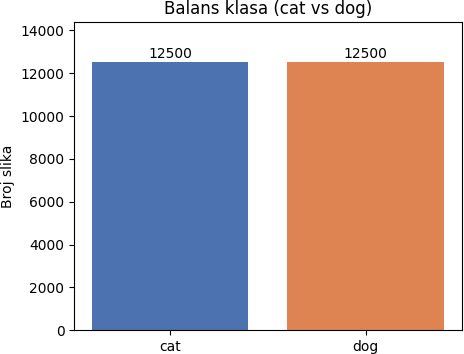
\includegraphics[width=0.9\textwidth]{img/balans.png}
    \end{figure}
\end{column}
\end{columns}
\end{frame}

\section{Baseline model}

\begin{frame}{Baseline --- VGG-6 treniran od nule}
\begin{columns}
\begin{column}{0.44\textwidth}
\begin{center}
\begin{tikzpicture}[
  node distance=2.6mm,
  box/.style={draw, rounded corners=1pt, minimum width=32mm, minimum height=4.6mm,
              font=\scriptsize, align=center, fill=blue!8},
  head/.style={box, fill=orange!20},
  arr/.style={-{Latex[length=1.4mm]}, gray}
]
\node[box] (a) {Ulaz 224$\times$224$\times$3};
\node[box, below=of a] (b) {Conv2D(32) + MaxPool};
\node[box, below=of b] (c) {Conv2D(64) + MaxPool};
\node[box, below=of c] (d) {Conv2D(128) + MaxPool};
\node[box, below=of d] (e) {Conv2D(128) + MaxPool};
\node[head, below=of e] (f) {Flatten $\rightarrow$ 25.088};
\node[head, below=of f] (g) {Dropout(0.5)};
\node[head, below=of g] (h) {Dense(512), ReLU};
\node[head, below=of h] (i) {Dense(1), Sigmoid};
\foreach \x/\y in {a/b,b/c,c/d,d/e,e/f,f/g,g/h,h/i} \draw[arr] (\x) -- (\y);
\end{tikzpicture}
\end{center}
\end{column}
\begin{column}{0.54\textwidth}
\begin{itemize}
    \item 4 bloka \texttt{Conv2D} + \texttt{MaxPooling2D}, filteri 3$\times$3, broj filtera raste 32\,$\rightarrow$\,64\,$\rightarrow$\,128\,$\rightarrow$\,128. \pause
    \item Ukupno \textbf{13.086.913} parametara. \pause
    \item \textbf{98\,\%} svih parametara je u jednom sloju --- \texttt{Dense(512)} posle \texttt{Flatten}-a (12.845.568). \pause
    \item Baš ta koncentracija kapaciteta je razlog zašto model lako \textbf{overfituje}. \pause
    \item Optimizator: RMSprop, \texttt{lr = 1e-4}; gubitak: Binary Crossentropy.
\end{itemize}
\end{column}
\end{columns}
\end{frame}

\begin{frame}{Baseline bez regularizacije --- demonstracija overfitovanja}
    \begin{figure}[h!]
        \begin{center}
          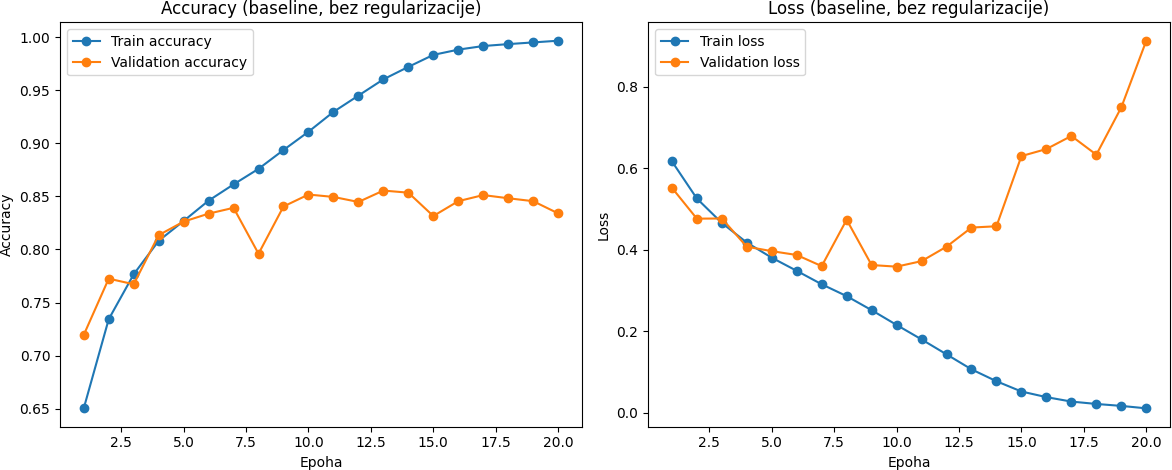
\includegraphics[width=0.86\textwidth]{img/baseline_overfit.png}
        \end{center}
       \caption{20 epoha, bez EarlyStopping-a --- namerno, da se overfitovanje vidi u celosti}
    \end{figure}
\vspace{-0.5\baselineskip}
\begin{itemize}
    \item Train accuracy \textbf{99,66\,\%}, validation accuracy \textbf{83,4\,\%} --- jaz od preko 16 poena.
    \item Validation loss \textbf{raste} sa 0,36 na 0,91 dok train loss pada ka nuli.
\end{itemize}
\end{frame}

\begin{frame}{Baseline sa regularizacijom}
    \begin{figure}[h!]
        \begin{center}
          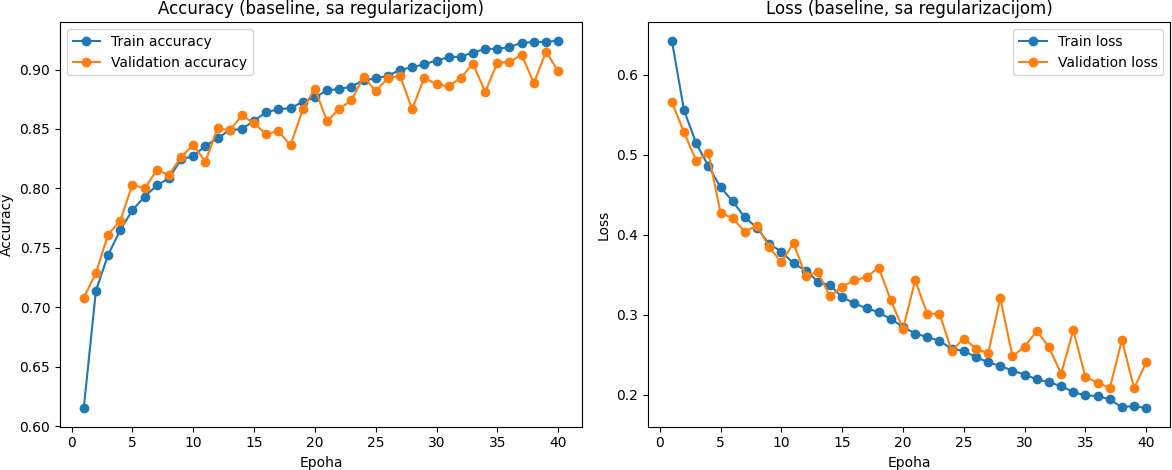
\includegraphics[width=0.86\textwidth]{img/baseline_reg.png}
        \end{center}
       \caption{Data augmentation + Dropout(0.5) + EarlyStopping}
    \end{figure}
\vspace{-0.5\baselineskip}
\begin{itemize}
    \item Isti optimizator i ista stopa učenja --- razlika dolazi \textbf{isključivo} od regularizacije.
    \item Krive ostaju blizu jedna drugoj: \textbf{test accuracy 90,30\,\%}.
\end{itemize}
\end{frame}

\section{Transfer learning}

\begin{frame}{Transfer learning sa VGG-16}
\begin{columns}
\begin{column}{0.44\textwidth}
\begin{center}
\begin{tikzpicture}[
  node distance=2.8mm,
  box/.style={draw, rounded corners=1pt, minimum width=34mm, minimum height=4.6mm,
              font=\scriptsize, align=center, fill=blue!8},
  froz/.style={box, fill=gray!22},
  head/.style={box, fill=orange!20},
  arr/.style={-{Latex[length=1.4mm]}, gray}
]
\node[box] (a) {Ulaz 224$\times$224$\times$3};
\node[box, below=of a] (b) {Data augmentation};
\node[box, below=of b] (c) {\texttt{preprocess\_input}};
\node[froz, below=of c] (d) {VGG-16 baza --- \textbf{zamrznuta}\\ $\rightarrow$ 7$\times$7$\times$512};
\node[head, below=of d] (e) {GlobalAveragePooling2D $\rightarrow$ 512};
\node[head, below=of e] (f) {Dense(256), ReLU};
\node[head, below=of f] (g) {Dropout(0.5)};
\node[head, below=of g] (h) {Dense(1), Sigmoid};
\foreach \x/\y in {a/b,b/c,c/d,d/e,e/f,f/g,g/h} \draw[arr] (\x) -- (\y);
\end{tikzpicture}
\end{center}
\end{column}
\begin{column}{0.54\textwidth}
\begin{itemize}
    \item VGG-16 sa ImageNet težinama, \texttt{include\_top=False} --- originalni klasifikator se odbacuje. \pause
    \item \textbf{Zašto zamrznuta baza:} nova glava ima nasumične težine i proizvodi ogromne gradijente koji bi u prvim koracima uništili naučene ImageNet težine. \pause
    \item \textbf{GlobalAveragePooling} umesto \texttt{Flatten}-a --- inače bi glava opet imala milione parametara. \pause
    \item Trenira se svega \textbf{131.585} od 14.846.273 parametara --- \textbf{manje od 1\,\%}. \pause
    \item Adam, \texttt{lr = 1e-3}, EarlyStopping i ReduceLROnPlateau.
\end{itemize}
\end{column}
\end{columns}
\end{frame}

\begin{frame}{Transfer learning --- tok treninga}
    \begin{figure}[h!]
        \begin{center}
          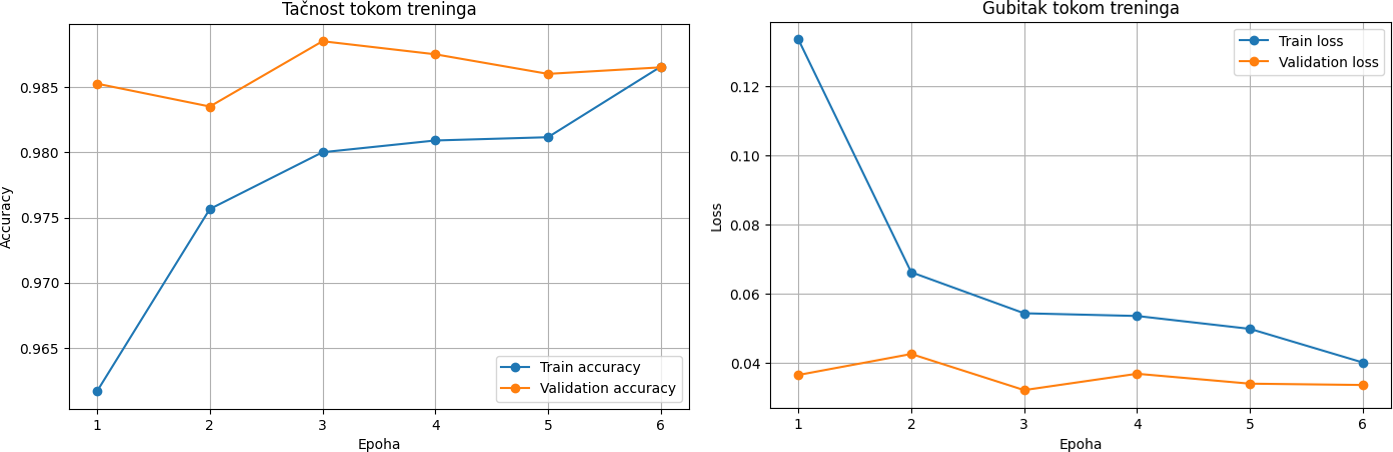
\includegraphics[width=0.92\textwidth]{img/tl_krive.png}
        \end{center}
    \end{figure}
\vspace{-0.5\baselineskip}
\begin{itemize}
    \item Već posle \textbf{prve epohe} validation accuracy je \textbf{98,52\,\%}.
    \item EarlyStopping staje u 6. epohi i vraća težine iz 3. epohe (najbolji \texttt{val\_loss}).
    \item \textbf{Test accuracy: 98,10\,\%} --- broj grešaka pao je sa 97 na 19.
\end{itemize}
\end{frame}

\section{Fine-tuning}

\begin{frame}{Fine-tuning VGG-16 modela}
\begin{itemize}
    \item Polazi se od sačuvanog transfer learning modela --- ne trenira se ništa iznova. \pause
    \item Odmrznut je \textbf{samo poslednji konvolucioni blok} (\texttt{block5\_conv1/2/3}): \pause
    \begin{itemize}
        \item niži slojevi uče \textbf{univerzalne} karakteristike (ivice, teksture) --- nema šta da se popravi, a ima šta da se pokvari \pause
        \item viši slojevi uče \textbf{semantiku specifičnu za ImageNet} --- tu prilagođavanje ima smisla \pause
        \item odmrzavanje cele baze značilo bi 14,7 miliona parametara na 20.000 slika \pause
    \end{itemize}
    \item Trenabilnih parametara: \textbf{7.211.009}; zamrznutih: 7.635.264. \pause
    \item Stopa učenja \textbf{1e-5} --- sto puta manja nego u prethodnoj fazi, jer se sada menjaju težine koje su \textbf{već dobre} (rizik od katastrofalnog zaboravljanja). \pause
    \item Model se mora \textbf{ponovo kompajlirati} da bi Keras primetio promenu \texttt{trainable} statusa.
\end{itemize}
\end{frame}

\begin{frame}{Fine-tuning --- tok treninga}
    \begin{figure}[h!]
        \begin{center}
          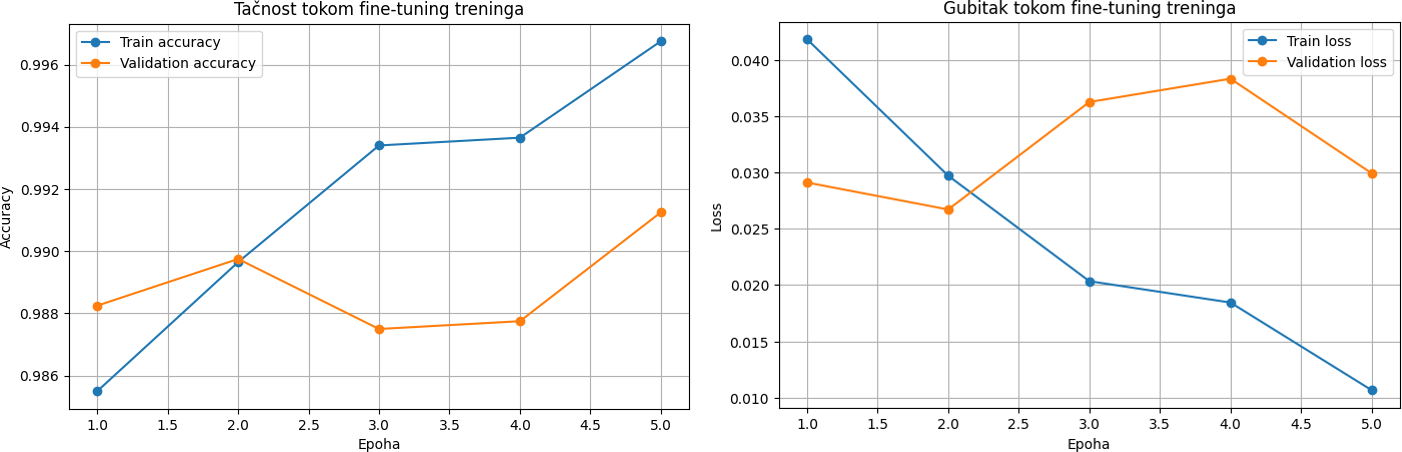
\includegraphics[width=0.92\textwidth]{img/ft_krive.png}
        \end{center}
    \end{figure}
\vspace{-0.5\baselineskip}
\begin{itemize}
    \item Najbolji \texttt{val\_loss} već u \textbf{2. epohi} (0,0267).
    \item Zatim train accuracy raste, a \texttt{val\_loss} se pogoršava --- početak overfitovanja; EarlyStopping staje u 5. epohi i vraća težine iz 2.
    \item \textbf{Test accuracy: 99,00\,\%}.
\end{itemize}
\end{frame}

\section{Rezultati}

\begin{frame}{Poređenje modela na test skupu}
    \begin{figure}[h!]
        \begin{center}
          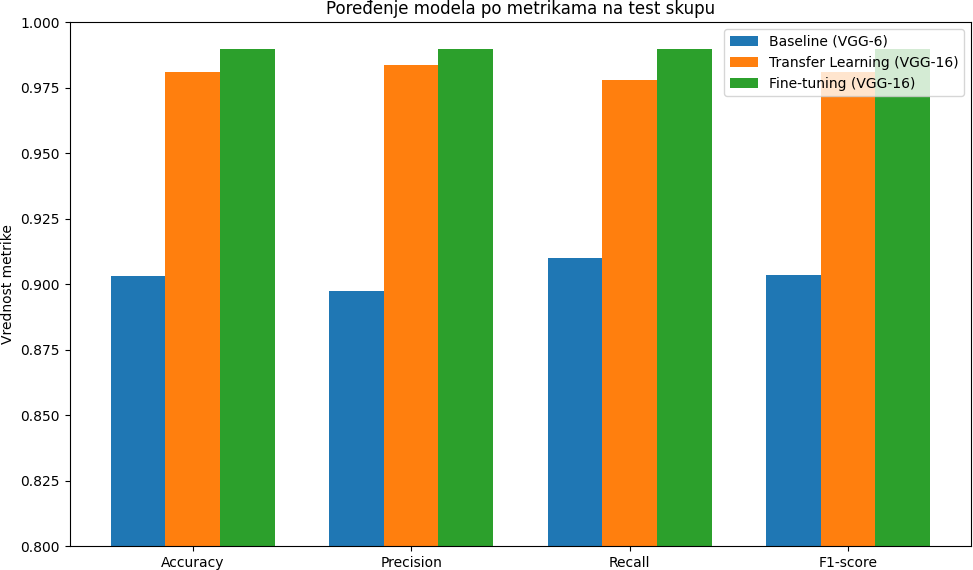
\includegraphics[width=0.62\textwidth]{img/poredjenje.png}
        \end{center}
    \end{figure}
\vspace{-0.7\baselineskip}
\begin{table}
\centering
\setlength{\tabcolsep}{4pt}
\begin{tabular}{lrrrrr}
\toprule
\textbf{Model} & \textbf{Accuracy} & \textbf{Precision} & \textbf{Recall} & \textbf{F1} & \textbf{Grešaka} \\
\midrule
Baseline VGG-6            & 90,30\,\% & 89,74\,\% & 91,00\,\% & 90,37\,\% & 97 \\
VGG-16 Transfer Learning  & 98,10\,\% & 98,39\,\% & 97,80\,\% & 98,09\,\% & 19 \\
\textbf{VGG-16 Fine-tuning} & \textbf{99,00\,\%} & \textbf{99,00\,\%} & \textbf{99,00\,\%} & \textbf{99,00\,\%} & \textbf{10} \\
\bottomrule
\end{tabular}
\end{table}
\end{frame}

\begin{frame}{Matrice konfuzije}
    \begin{figure}[h!]
        \begin{center}
          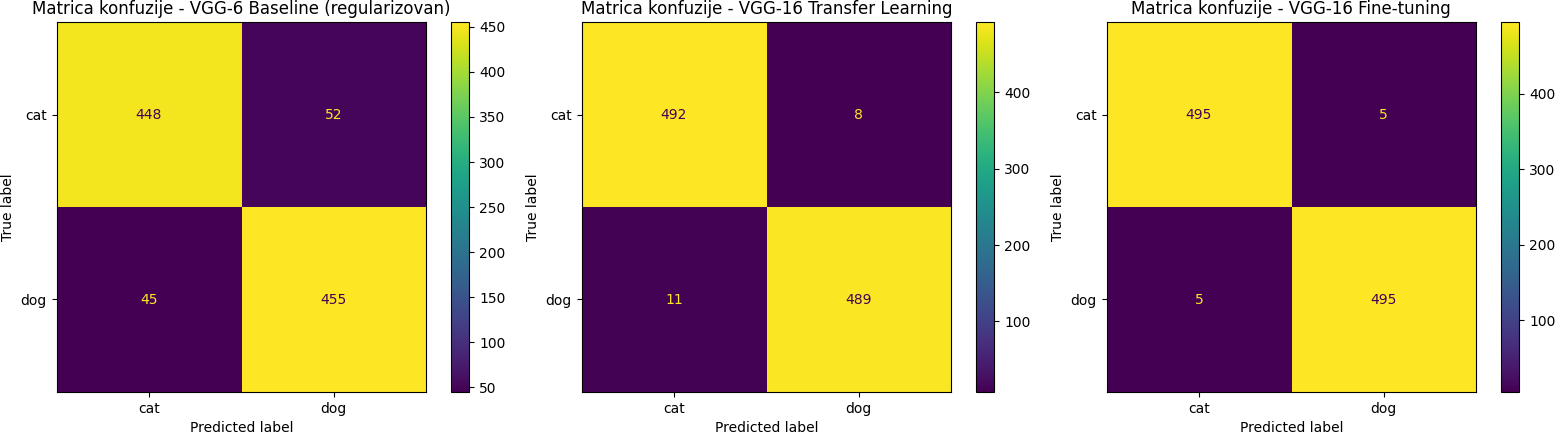
\includegraphics[width=0.98\textwidth]{img/cm_sve.png}
        \end{center}
       \caption{Baseline \quad$\vert$\quad Transfer learning \quad$\vert$\quad Fine-tuning}
    \end{figure}
\vspace{-0.5\baselineskip}
\begin{itemize}
    \item Greške su u sva tri modela \textbf{simetrične} --- nema pristrasnosti ka jednoj klasi.
    \item Kod finalnog modela po \textbf{5 grešaka} sa svake strane, pa su sve četiri metrike identične.
    \item \textbf{Ograničenje:} razlika 98,10\,\% naspram 99,00\,\% je 9 slika od 1.000 --- nije statistički čvrsto dokazana.
\end{itemize}
\end{frame}

\section{Interpretabilnost}

\begin{frame}{Interpretabilnost --- međuslojne aktivacije}
\vspace{-0.3\baselineskip}
\begin{itemize}
    \item Model sa 99\,\% tačnosti i dalje može biti tačan \textbf{iz pogrešnog razloga} (klasifikator vukova koji je detektovao sneg u pozadini).
    \item Dva komplementarna pristupa: \textbf{aktivacije} --- šta mreža računa; \textbf{Grad-CAM} --- zašto je odlučila baš tako.
\end{itemize}
\vspace{-0.3\baselineskip}
\begin{figure}[h!]
    \begin{center}
      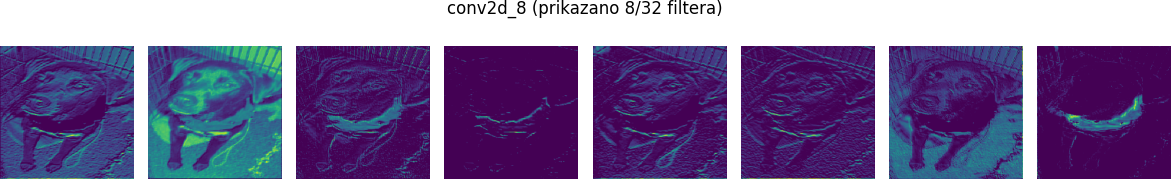
\includegraphics[width=0.8\textwidth]{img/akt_plitko.png}\\[1mm]
      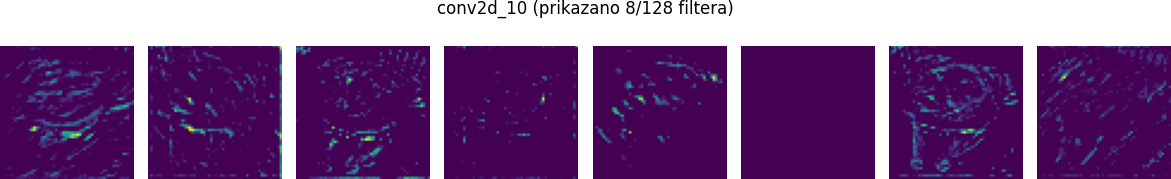
\includegraphics[width=0.8\textwidth]{img/akt_duboko.png}
    \end{center}
   \caption{Prvi (gore) i treći (dole) konvolucioni sloj: detektori ivica $\rightarrow$ apstraktne reprezentacije}
\end{figure}
\end{frame}

\begin{frame}{Retkost (sparsity) aktivacija po sloju}
\begin{columns}
\begin{column}{0.55\textwidth}
    \begin{figure}[h!]
        \centering
        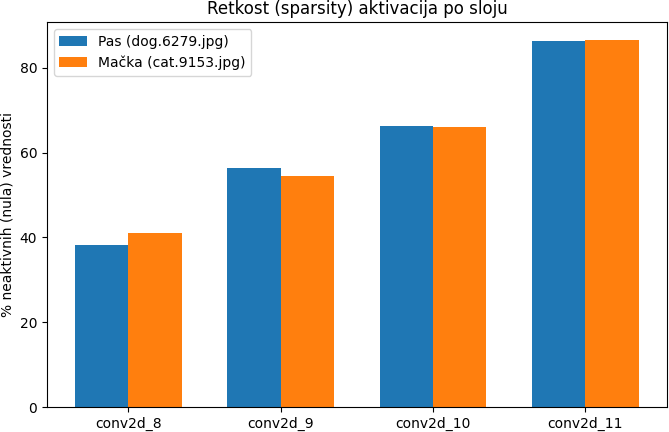
\includegraphics[width=\textwidth]{img/sparsity.png}
    \end{figure}
\end{column}
\begin{column}{0.43\textwidth}
\begin{itemize}
    \item Udeo tačnih nula (posledica ReLU aktivacije) raste sa dubinom: \textbf{38--41\,\%} u prvom sloju do \textbf{86--87\,\%} u poslednjem. \pause
    \item Gotovo \textbf{identično za obe klase} --- dakle opšte svojstvo mreže, a ne nešto specifično za mačke i pse. \pause
    \item Uočen je i jedan potpuno neaktivan filter --- verovatno \textit{dead ReLU}.
\end{itemize}
\end{column}
\end{columns}
\end{frame}

\begin{frame}{Grad-CAM --- kako radi}
\begin{itemize}
    \item \textit{Gradient-weighted Class Activation Mapping} (Selvaraju i sar., 2017) --- toplotna mapa oblasti koje su najviše doprinele konkretnoj odluci. \pause
    \item Postupak:
    \begin{enumerate}
        \item uzme se izlaz poslednjeg konvolucionog sloja \texttt{block5\_conv3} (\textbf{14$\times$14$\times$512}) \pause
        \item izračunaju se gradijenti skora klase po tim mapama i \textbf{prostorno usrednje} --- dobija se težina po kanalu \pause
        \item težinska suma mapa, pa \textbf{ReLU} (zadržavaju se samo pozitivni doprinosi) \pause
        \item normalizacija i uveličavanje na dimenzije slike \pause
    \end{enumerate}
    \item \textbf{Dve implementacione odluke:} \pause
    \begin{itemize}
        \item Grad-CAM se računa nad \textbf{logitom}, ne nad izlazom sigmoide --- kod sigurnih predikcija sigmoida je zasićena i gradijenti bi nestali \pause
        \item za klasu \texttt{cat} koristi se \textbf{$-$logit}, jer jedini izlazni neuron meri „koliko je ovo pas''
    \end{itemize}
\end{itemize}
\end{frame}

\begin{frame}{Grad-CAM --- rezultati}
\begin{columns}
\begin{column}{0.5\textwidth}
    \begin{figure}[h!]
        \centering
        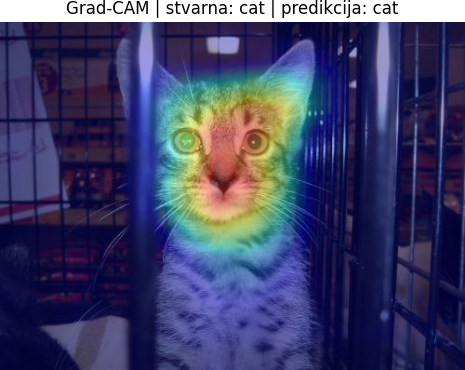
\includegraphics[height=42mm]{img/gradcam_cat.png}
    \end{figure}
\end{column}
\begin{column}{0.5\textwidth}
    \begin{figure}[h!]
        \centering
        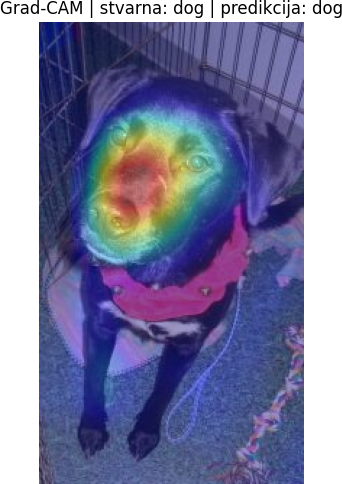
\includegraphics[height=42mm]{img/gradcam_dog.png}
    \end{figure}
\end{column}
\end{columns}
\vspace{0.3\baselineskip}
\begin{itemize}
    \item Model se fokusira na \textbf{glavu, oči i njušku}, a pozadina ostaje hladna.
    \item Odluke se zasnivaju na samoj životinji --- \textbf{nema „Clever Hans'' efekta}.
    \item \textbf{Ograničenje:} analiza je kvalitativna, na šest primera; za tvrd zaključak bila bi potrebna kvantitativna mera nad celim test skupom.
\end{itemize}
\end{frame}

\section{Demonstracija}

\begin{frame}{Demo --- kompletan tok}
\begin{columns}
\begin{column}{0.45\textwidth}
    \begin{figure}[h!]
        \centering
        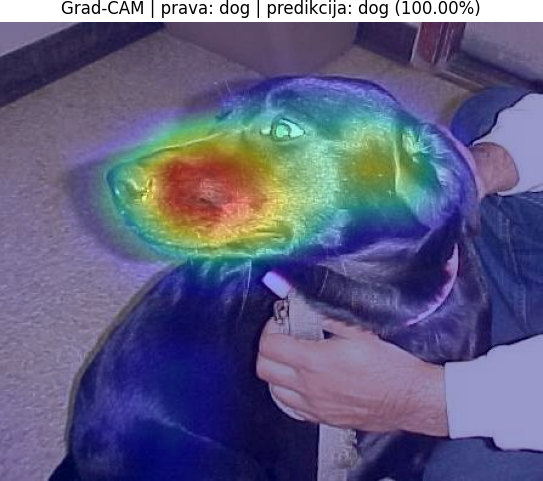
\includegraphics[width=\textwidth]{img/demo.png}
    \end{figure}
\end{column}
\begin{column}{0.53\textwidth}
\begin{itemize}
    \item Učitavanje finalnog modela \texttt{vgg16\_finetuned.keras}. \pause
    \item Slika se skalira na 224$\times$224 i prosleđuje modelu --- \textbf{bez ručne pripreme}, jer \texttt{preprocess\_input} radi unutar samog modela. \pause
    \item Izlaz: predviđena klasa i pouzdanost. \pause
    \item Grad-CAM objašnjava \textbf{zašto} je model tako odlučio.
\end{itemize}
\end{column}
\end{columns}
\end{frame}

\section{Zaključak}

\begin{frame}{Zaključak}
\begin{itemize}
    \item Prethodno naučeno znanje vredi više od kapaciteta modela: transfer learning trenira \textbf{100 puta manje parametara} od baseline-a, a smanjuje broj grešaka za \textbf{80\,\%}. \pause
    \item Fine-tuning poslednjeg bloka donosi dodatno poboljšanje --- finalnih \textbf{99,00\,\%} na test skupu. \pause
    \item Jedinstvena podela iz \texttt{split.csv} omogućila je da se razlike pripišu \textbf{modelu}, a ne sreći u podeli podataka. \pause
    \item Interpretabilnost potvrđuje da je model tačan \textbf{iz pravog razloga} --- gleda životinju, ne pozadinu. \pause
    \item Pravci za dalji rad: veći test skup ili unakrsna validacija, poređenje sa modernijim arhitekturama, i kvantitativna Grad-CAM analiza.
\end{itemize}
\end{frame}

\begin{frame}
    \vfill
    \centering
    \Huge Hvala na pažnji!
    \vfill
\end{frame}

\end{document}
